\section{The ANNs }
The Artificial Neural Network used for this project was a modified ANN from Dr. Pyeatte's code. We converted his ANN to python and removed the back-propagation function and saving and loading from files. We added a mutation function and a recombination function. The mutation function takes the number of weights that are to be mutated then randomly chooses that number of weights and randomly assigns them a value. The recombination function takes to lists of weights as arguments and gives a 50-50 chance of choosing a weight from one or the other to create its own weights.
\\
\\
Each AI contains a neural network for each role card that can be chosen. So there is one for the captain, trader, settler, builder, mayor, craftsman, and prospector. Each one of these phases take the same number of inputs, however they have different outputs because of the different things that are accomplished in each phase.
\subsection{The Inputs}
Each phase takes the entire game board as inputs. Player 1's colonists, buildings, plantations, victory points, doubloons, goods, and player 3 and player 2 inputs. Also what is currently on the trade ship, cargo ship, colonists ship, victory points remaining, colonists left, and doubloons left as well are all inputs to each phase.
\subsection{The Outputs}
The difference between the phases lies with the outputs. Since each phase allows a player to do something else, the outputs needed to be different. For example the building phase outputs would be the possible buildings that the player can buy. They would be ranked from highest to lowest. The player would start with the highest building that the ANN outputted and try to buy it. If it doesn't have enough doubloons it would go to the next highest ranked building. This will continue until a building is bought or the next highest building is buy nothing option.The same thing would happen with other phases where it will try to do the highest ranked output.
\subsection{Example ANN}
See Figure~\ref{ANN Example}.  This is an example of a building phase ANN. The whole game board is given as inputs to the neural network. The number of colonists, each building and plantation type, number of each resource, victory points, and the amount of dabloons they have are all given under the player inputs. Player1 inputs used to save space in the figure. All of this information fed through the hidden layers and then outputs in the building phase are ranked. The higher the output the better the option is. The player will start with the best ranked option and try to do it. If it doesn't have enough dabloons to buy it the next option is chosen and repeats until something is bought or buy nothing is chosen.
\begin{figure}[tbh]
\begin{center}
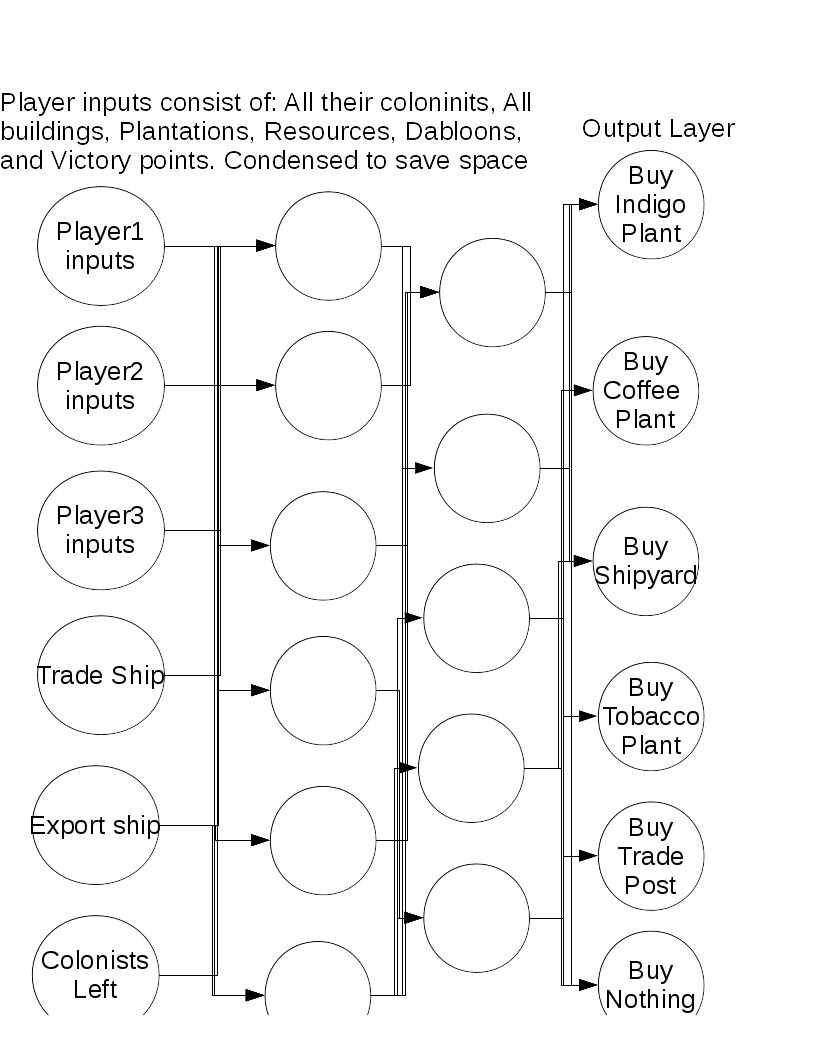
\includegraphics[width=0.75\textwidth]{./images/Example_ANN.png}
\end{center}
\caption{A example of a building phase ANN \label{ANN Example}}
\end{figure}
